% !TeX root = ../main.tex

\chapter{Related Work}\label{chapter:RelatedWork}

\section{Virtual Embodiment: Dealing with Discrepancies between the Virtual and the Real Body}

In his thesis \textit{Virtual Embodiment:  Dealing with Discrepancies between the Virtual and the Real Body} \autocite{JohnnyVEThesis} Jonathan Haudenschild proposed and implemented various feedback mechanisms to deal with such discrepancies in room-scale \gls{vra}. He focused on ideas that rely only on the basic \textit{HTC Vive} hardware, namely the two \glspl{controllergl} and the \gls{hmda}.
\newline
His work forms the basis of this thesis, with the addition of a fully tracked body, utilising some new hardware, \textit{Vive Trackers}, discussed in \autoref{chapter:Hardware}. The focus is shifted from discrepancies only at hands and head to also include the user's tracked feet, as well as implementing all feedback mechanisms into a \gls{vra} client for the \textit{Neurorobotics Platform}, which will be presented in \autoref{chapter:Software}.
\newline

Haudenschild proposes various feedback mechanisms to notify the user of, and encourage him to correct, situations in which he has a pose or is in a position his virtual body should physically not be, which results in discrepancies.
\newline
For discrepancies at the head, such as when the user sticks his head into a wall, he implemented multiple visual effects \autocite[p. ~20]{JohnnyVEThesis}:
\begin{itemize}
    \item Blurring the user's view
    \item Distorting the user's view
    \item Changing the colours of everything in the user's view
    \item Fading the user's view to black
    \item Rendering the insides of objects with highlighted edges.
\end{itemize}
For discrepancies at the hand, for instance when the user places his hand into an object, he implemented visual, haptic, and auditory effects \autocite[p. ~24-25]{JohnnyVEThesis}:
\begin{itemize}
    \item A ghost image of the user's hand, which follows his real, tracked hand into objects and is visible inside them
    \item Lines connecting the tracked and physically simulated hand
    \item Vibrating the controller
    \item Playing a sound at the position of the user's hand.
\end{itemize}

In his user study, it was found that, for discrepancies at the hand, the haptic feedback provided by vibrating the controller, as well as seeing the ghost image of the user's real hands were most helpful in resolving or avoiding discrepancies, as well as increasing the participants' \gls{immersiongl}. The sound feedback was found to be not only barely helpful, but also proved negatively impacting on \gls{immersiongl} \autocite[p. ~29-34]{JohnnyVEThesis}.
\newline
Concerning discrepancies at the head, the most obvious finding was that the distortion effect was not well received by participants, the blur effect was received best, and the colour change effect, as well as the fade to black effect, had mixed reception. Rendering the interior of objects was mainly effective at preventing users from seeing through walls, and fulfils a different role than the other effects, which also encourage the user to resolve the discrepancy. It was suggested to combine the blur and fade to black effects at lower intensity, as well as using the colour change effect more subtly, merely to notify the user about discrepancies  \autocite[p. ~35-39]{JohnnyVEThesis}.

\section{Real-Time Body Tracking in Virtual Reality using a Vive Tracker}

Polona Caserman et al. in their article \textit{Real-Time Body Tracking in Virtual Reality using a Vive Tracker} \autocite{bodyTrackingVR} evaluated currently used methods of full body tracking in \gls{vra}, namely \textit{Microsoft Kinect}\footnote{Microsoft Kinect: \url{https://developer.microsoft.com/en-us/windows/kinect}}, systems using multiple cameras with a motion capture suit such as \textit{OptiTrack}\footnote{OptiTrack: \url{https://optitrack.com/}}, and systems using \glspl{imua} attached to limbs, such as \textit{PrioVR}\footnote{PrioVR: \url{https://yostlabs.com/priovr/}} (\autoref{fig:bodyTrackingSystems}).

\begin{figure}[h]
    \centering
    \subfloat[MS Kinect 2][Microsoft Kinect 2 \autocite{kinectPic}]{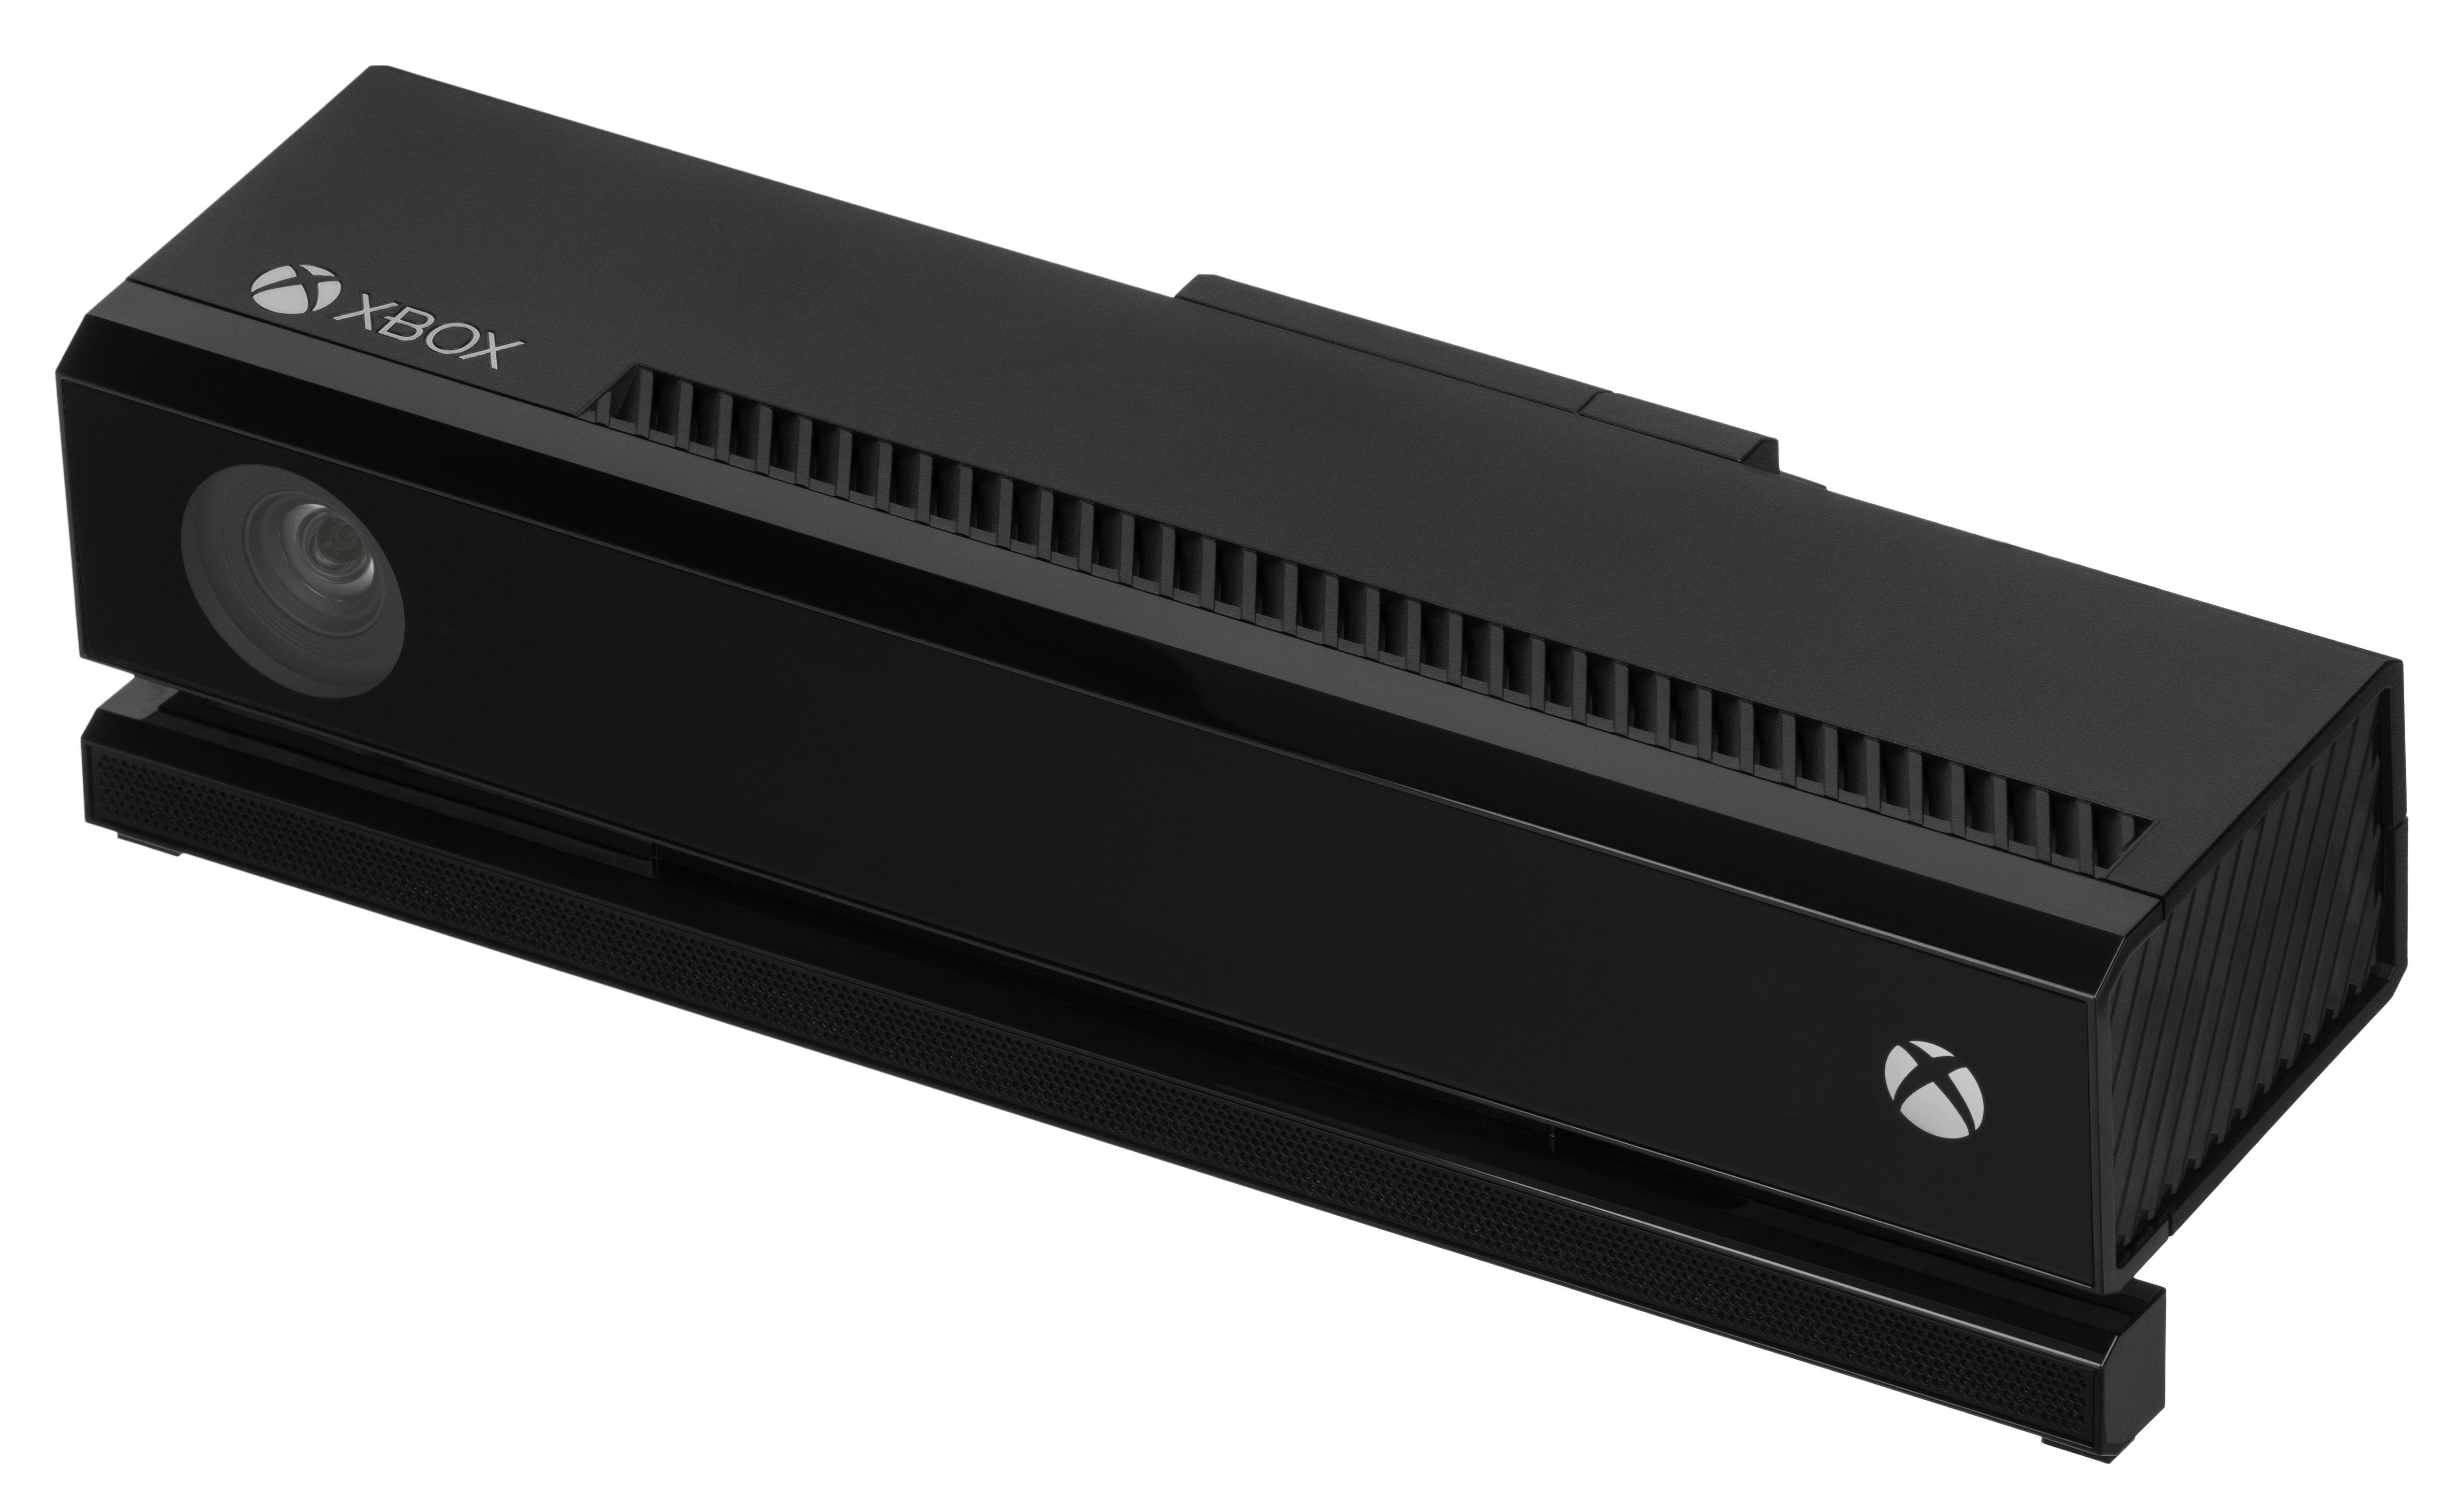
\includegraphics[width=0.3\textwidth]{figures/Xbox-One-Kinect}\label{fig:kinect}}
    \hfill
    \subfloat[PrioVR][PrioVR diagram \autocite{prioVRDiagram}]{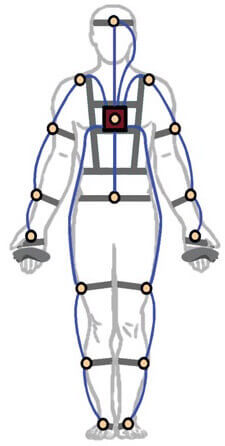
\includegraphics[width=0.15\textwidth]{figures/priovr-suit-diagram}\label{fig:prioVR}}
    \hfill
    \subfloat[OptiTrack][OptiTrack diagram
    \autocite{optiTrackPic}]{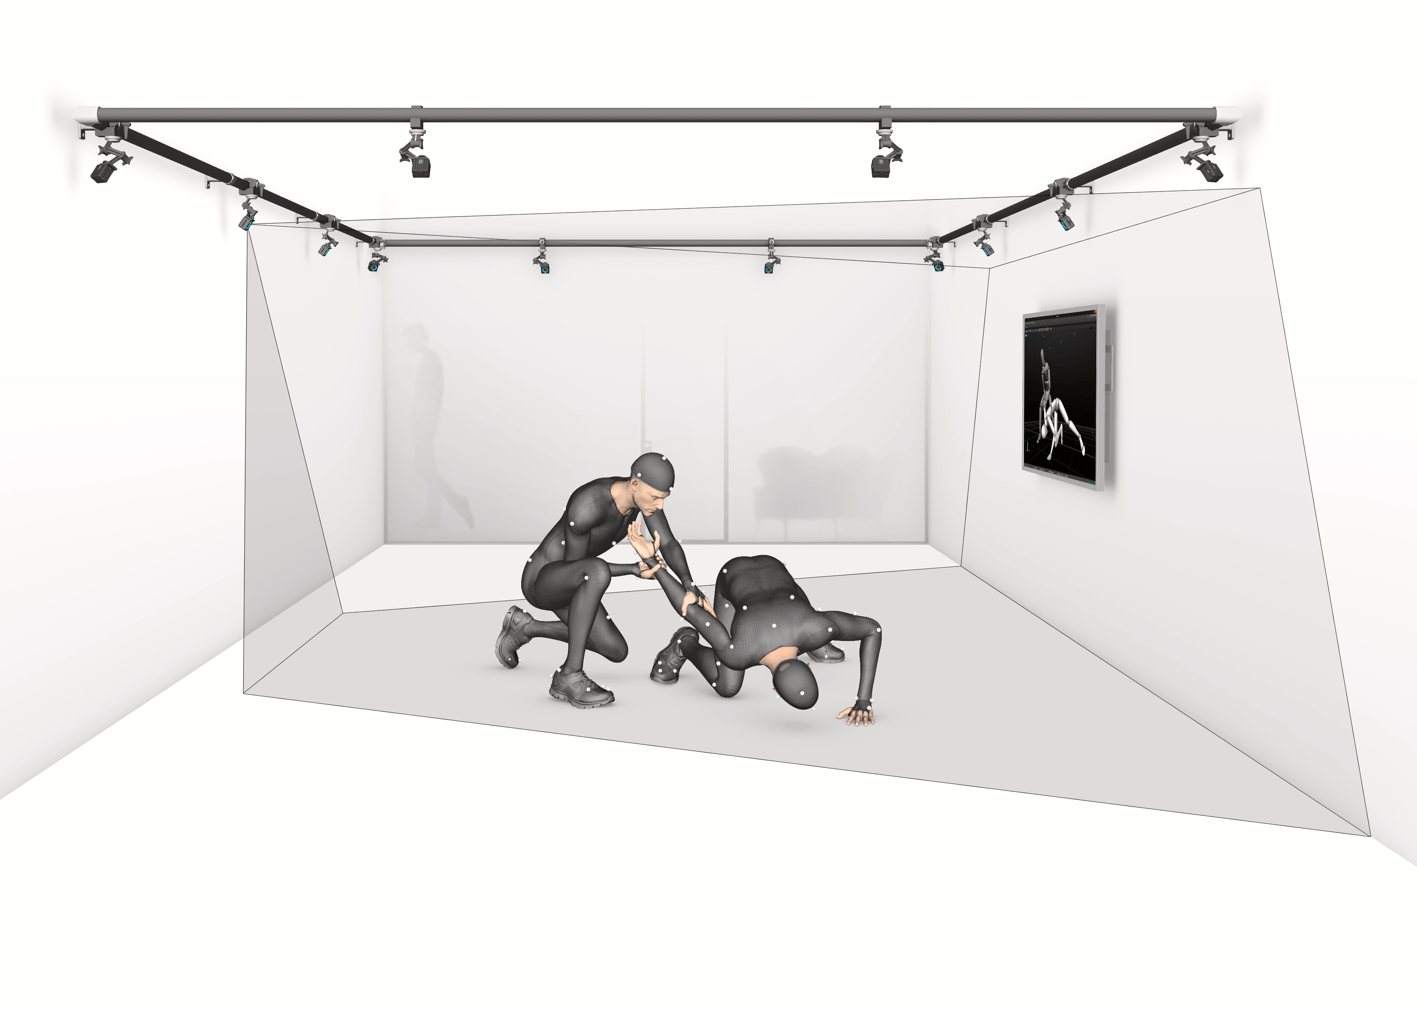
\includegraphics[width=0.45\textwidth]{figures/conference-room-volume@2x}\label{fig:optiTrack}}
    \caption{Full Body Tracking Systems}
    \label{fig:bodyTrackingSystems}
\end{figure}

They found that while \enquote{the Kinect suffers from occlusion, provides
noise in skeleton tracking and has a high latency} \autocite[p. ~3]{bodyTrackingVR} it is used in many applications for which it provides adequate accuracy due to its low cost and ease of use.
\newline
On the other hand, \enquote{a wearable motion capture suit is capable of a very accurate body tracking. However, it is very expensive and complicated to use} and as such \enquote{not applicable for home-based usage}  \autocite[p. ~3]{bodyTrackingVR}.
\newline
The authors also favourably mention systems using \glspl{imua}, without analysing latency or cost. For their research they decided to use \textit{Vive Trackers} attached to hands and feet, with the pose of the body calculated based on the position and rotation of the trackers using \gls{ika}.


\section{You Shall Not Pass: Non-Intrusive Feedback for Virtual Walls in VR Environments with Room-Scale Mapping}\label{section:YouShallNotPass}

In their thesis \textit{You Shall Not Pass: Non-Intrusive Feedback for Virtual Walls in VR Environments with Room-Scale Mapping} \autocite{nonIntrusiveFeedback}, a team of researchers around M. Boldt investigated methods of making the user respect virtual boundaries, such as walls in room-scale \gls{vra}.
\newline
They began by analysing if and how commercial VR applications handle situations in which the user could interact with walls. Only one application, namely \textit{Nvidia VR Funhouse}, \enquote{provides vibrotactile feedback when interacting with big game elements. However, it features neither auditory nor visual feedback.} \autocite[p. ~1]{nonIntrusiveFeedback}. None of the other tested games provided any sensory feedback in such situations.
\newline
Another observation was that only one tested game (\textit{The Lab}) had walls which had two-side rendered planes, meaning that in all other games, when the camera moved through a wall, the backside of it would be invisible, allowing the user to see through it.
\newline
It was found that \enquote{most state of the art VR games either (1) stop the game progress and limit rewards or otherwise punish the player using game mechanics when crossing walls, (2) are designed in a way so the players cannot get close to the walls at all, or (3) simply avoid walls completely within the play area} \autocite[p. ~2]{nonIntrusiveFeedback}. The conclusion was that most \gls{vra} applications are designed to simply avoid situations in which the user can interact with walls.
\newline

The researchers continue with presenting other research into collision feedback in \gls{vra}, some of which will be discussed further on.
\newline
The majority of the systems only provides haptic feedback, without visual or auditory components. They also rely on proprietary hardware, requiring \enquote{precise setup and calibration for every use} \autocite[p. ~2]{nonIntrusiveFeedback} which did not suit their use case. An exception to this is the \textit{simulated surface constraints technique}, which stops the virtual hand from penetrating the object, introducing a discrepancy between the virtual and real hand. It is claimed that \enquote{users are more sensitive to noticing hand-object penetration} \autocite[p. ~3]{nonIntrusiveFeedback} than such discrepancies.
\newline

The feedback mechanisms implemented in their experiment are:
\begin{itemize}
    \item for \gls{hmda}-wall collisions: black vision as visual feedback, and  muffled background music as auditory feedback;
    \item for \gls{controllergl}-wall collisions: a knocking sound as auditory feedback, and vibration as tactile feedback.
\end{itemize}
In the experiment it was found that in the control group, significantly more participants walked through walls, compared to the participants which had the feedback mechanisms enabled. It was also found that having the auditory and tactile feedback on \gls{controllergl}-wall collisions deterred many participants from even attempting to walk through walls, as well as the visual feedback on \gls{hmda}-wall collisions causing many, who did attempt to move through walls anyway, to step back and decide not to pass through \autocite[p. ~6,7]{nonIntrusiveFeedback}.



\section{Impacto: Simulating Physical Impact by Combining Tactile Stimulation with Electrical Muscle Stimulation} \label{section:impacto}

Pedro Lopes, Alexandra Ion, and Patrick Baudisch present a device they call \textit{impacto}, \enquote{designed to render the haptic
sensation of hitting and being hit in virtual reality} \autocite[p. ~1]{impacto} in their paper \textit{Impacto: Simulating Physical Impact by Combining Tactile Stimulation with Electrical Muscle Stimulation} \autocite{impacto}.
\newline

\begin{figure}[h]
    \centering
    \subfloat[impactoHand][Attached to arm, simulating being hit by a boxer ]{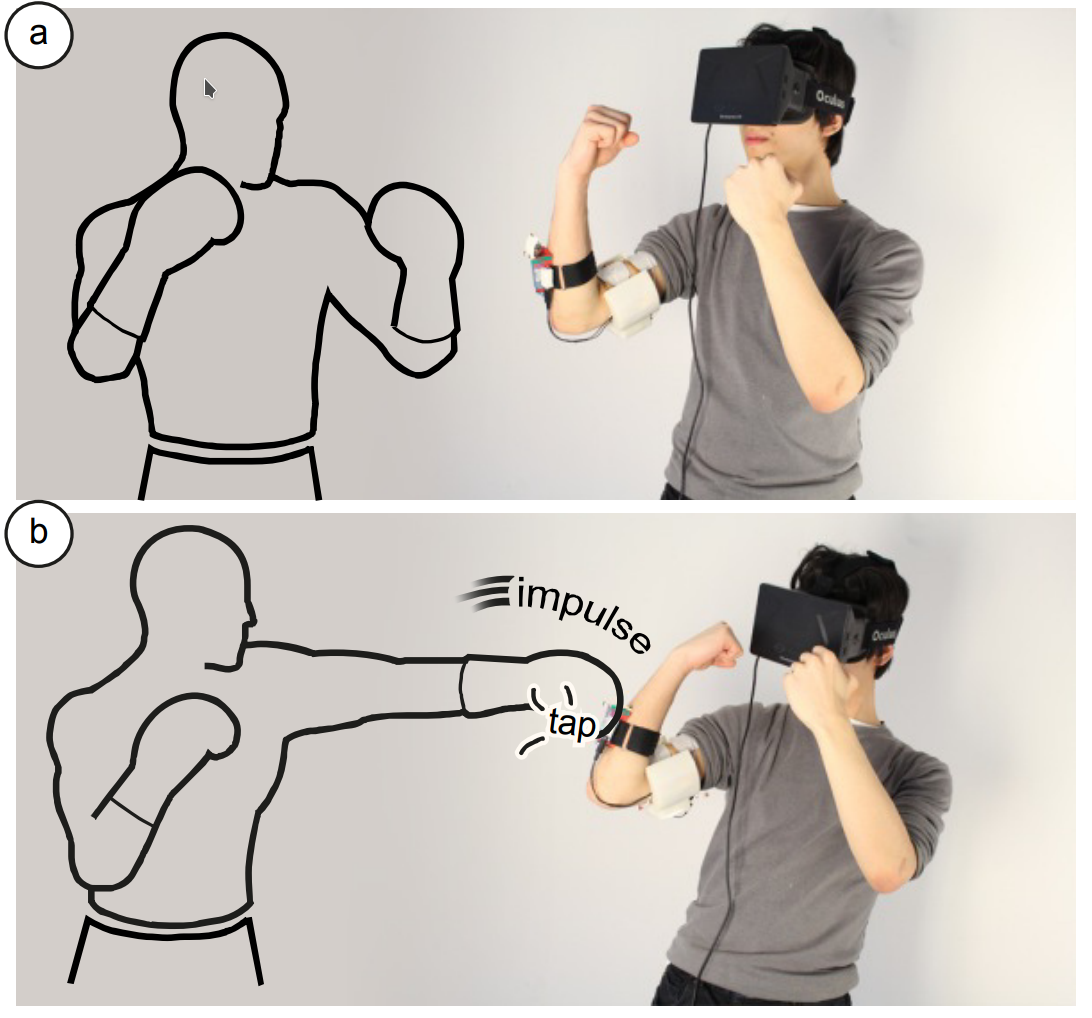
\includegraphics[width=0.3\textwidth]{figures/impactoHand}\label{fig:impactoHand}}
    \hfill
    \subfloat[impactoFoot][Attached to leg, simulating kicking a ball]{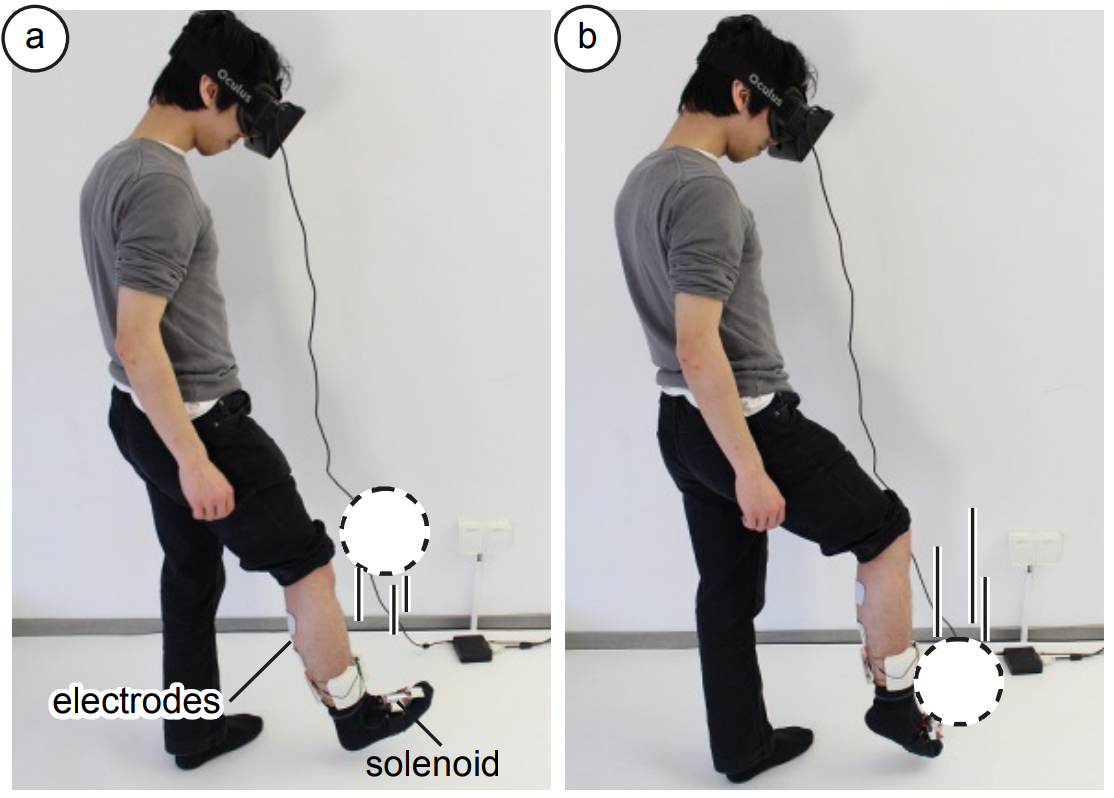
\includegraphics[width=0.3\textwidth]{figures/impactoFoot}\label{fig:impactoFoot}}
    \hfill
    \subfloat[impactoBat][Attached to arm and bat, simulating hitting a ball]{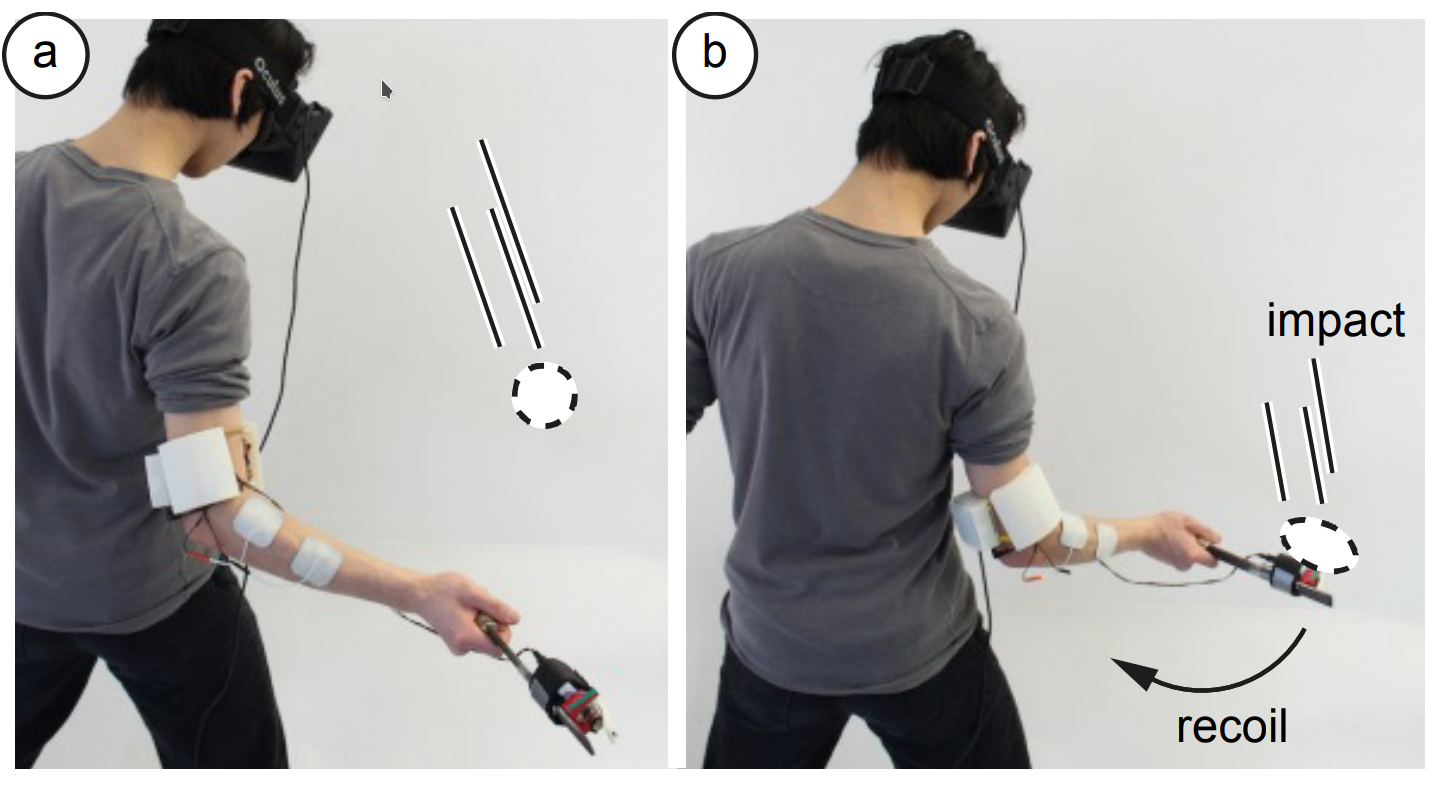
\includegraphics[width=0.3\textwidth]{figures/impactoBat}\label{fig:impactoBat}}
    \caption{\textit{Impacto} in various configurations \autocite{impacto}}
    \label{fig:impactoConfigs}
\end{figure}

The \textit{impacto} device is wireless and can be attached to a user's arms to create the sensation of being hit by creating a tactile stimulus using a solenoid, as well as simulating impulse by causing the arm to thrust backwards due to \gls{emsa} (Figure \autoref{fig:impactoHand}). Use on legs is also possible, enhancing the experience of kicking (Figure \autoref{fig:impactoFoot}), as well as use in combination with props, such as a bat (Figure \autoref{fig:impactoBat}). Multiple \textit{impacto} units can also be combined into a simple haptic suit.
\newline
A user study was conducted, in which it was found that each effect, \gls{emsa} and the solenoid hit, yielded increased perceived realism with increasing intensity of the effect individually, but the \enquote{highest
score, however, was achieved by combining both stimuli} \autocite[p. ~8]{impacto}.


\section{Providing Haptics to Walls \& Heavy Objects in Virtual Reality by Means of Electrical Muscle Stimulation}
                        
A similar approach to that discussed under \autoref{section:impacto} is taken in another paper by Pedro Lopes et al., \textit{Providing Haptics to Walls \& Heavy Objects in Virtual Reality by Means of Electrical Muscle Stimulation} \autocite{wallHaptics}, in which \gls{emsa} is used to create the sensation of heavy or immovable objects exerting force on a user's arms.
\newline
The method employed works by actuating opposing muscles in order to create a force in the direction an object would be exerting force on the user's arm, when interacting with the object. For example, picking up a heavy box requires the user's biceps to contract, so, depending on the object's weight, the user's triceps is actuated using \gls{emsa} with an appropriate intensity. This same principle is used for stationary objects, such as walls.
\newline
It was however found that preventing the user's hand from penetrating an object by applying a continuous opposing force \enquote{would draw the user’s attention to the EMS-actuated muscles} \autocite[p. ~2]{wallHaptics} due to it becoming arbitrarily strong the harder the user pushed against the object.
In response to this, two other approaches were implemented. The soft object design (Figure \autoref{fig:wallHapticsSoft}) allows users to penetrate objects with increasing resistance, creating the impression of soft objects. The other approach is the repulsion object design, \enquote{where the EMS propels the user’s hand backwards, removing it from the virtual object it is trying to touch} \autocite[p. ~3]{wallHaptics} (Figure \autoref{fig:wallHapticsRepulsive}).

\begin{figure}[h]
    \centering
    \subfloat[wallHapticsHard][Hard object design makes \gls{emsa} too obvious]{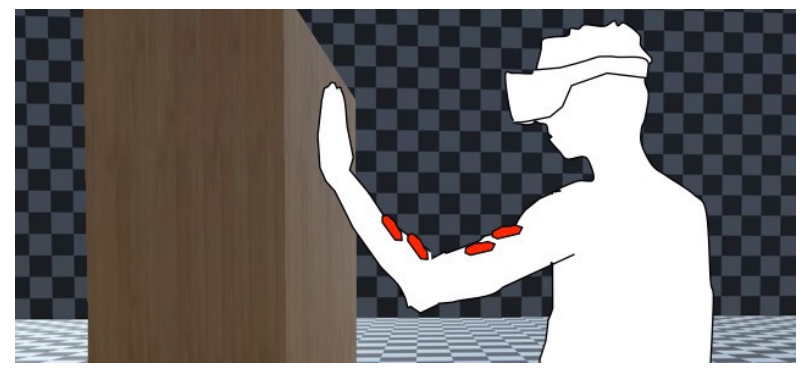
\includegraphics[width=0.3\textwidth]{figures/wallHapticsHand}\label{fig:wallHapticsHand}}
    \hfill
    \subfloat[wallHapticsSoft][Soft object design allows users to penetrate object with increasing resistance]{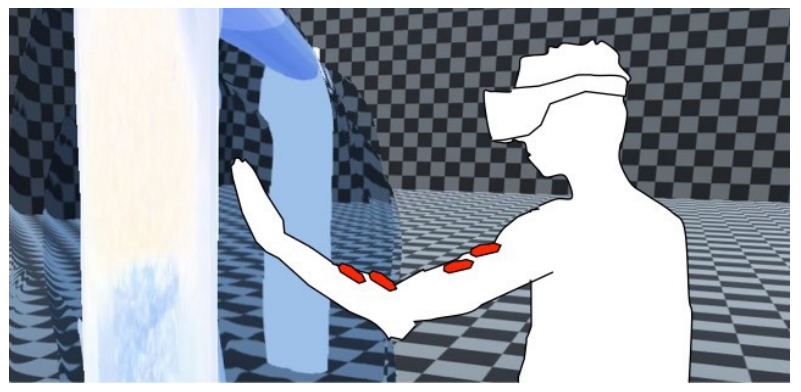
\includegraphics[width=0.3\textwidth]{figures/wallHapticsSoft.png}\label{fig:wallHapticsSoft}}
    \hfill
    \subfloat[wallHapticsRepulsive][Repulsion object design repels user's hand with a short impulse]{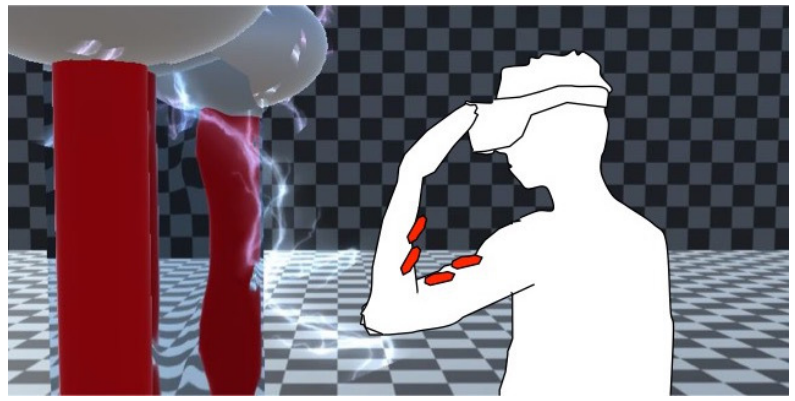
\includegraphics[width=0.3\textwidth]{figures/wallHapticsRepulsive.png}\label{fig:wallHapticsRepulsive}}
    \caption{Various approaches to stop object penetration \autocite{wallHaptics}}
    \label{fig:wallHapticsDesigns}
\end{figure}

In the user study, the repulsion object design was implemented with the so called \textit{electro} visuals. \enquote{This design complements the EMS pulse with a strong white flash which turns the screen white for 100 ms and then fades it back in in 100 ms. At the same time, users hear a loud electrical “bang”} \autocite[p. ~3]{wallHaptics}. In addition, a vibration motor suggests an electric shock to the user's hand. This object design was favoured by most participants, and was rated as most realistic.
\newline
The soft object design was implemented in two ways, one with visuals suggesting a magnetic field, another depicting a solid wooden wall. Of the two, the wooden version was preferred. The wall with the magnetic field however was rated as more realistic \autocite[p. ~4]{wallHaptics}. This suggests that the visual representation matching the type of force feedback is important in regard to perceived realism.
\newline
Both the soft and the repulsion object designs were considered significantly more impermeable than control objects, which only actuated the vibration motors on user's hands, whereby impermeability \enquote{shows participants’ assessment of
'this wall was able to prevent me from passing through'} \autocite[p. ~5]{wallHaptics}.


\section{Passive Haptics}\label{section:passiveHaptics}

In the context of virtual reality, \gls{pha} is a \enquote{technique that incorporates passive physical objects into virtual environments to physically simulate the virtual objects} \autocite[p. ~9]{passiveHaptics}. An example would be a sphere roughly the size of a virtual football. The user can pick up and manipulate the sphere, and the virtual football will move accordingly. In his PhD thesis, \textit{Passive haptics significantly enhances virtual environments}, Brent Edward Insko investigates the increase in \textit{presence} (a component of \gls{immersiongl}) of the user in a virtual environment, if said environment is recreated to mimic the virtual one with simple props in the real world.
\newline

\begin{figure}[h]
    \centering
    \subfloat[passiveHapticsVirtualRoom][Virtual environment]{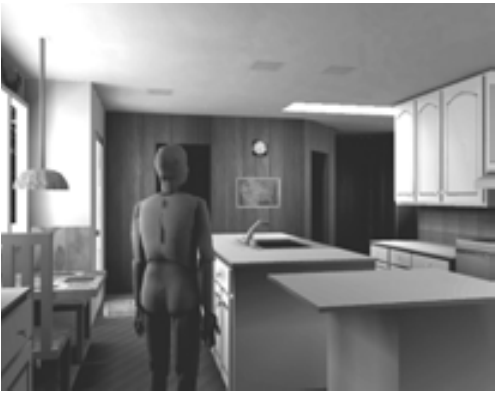
\includegraphics[width=0.3\textwidth]{figures/passiveHapticsVirtualRoom}\label{fig:passiveHapticsVirtualRoom}}
    \hfill
    \subfloat[passiveHapticsRealRoom][Real environment with low detail props]{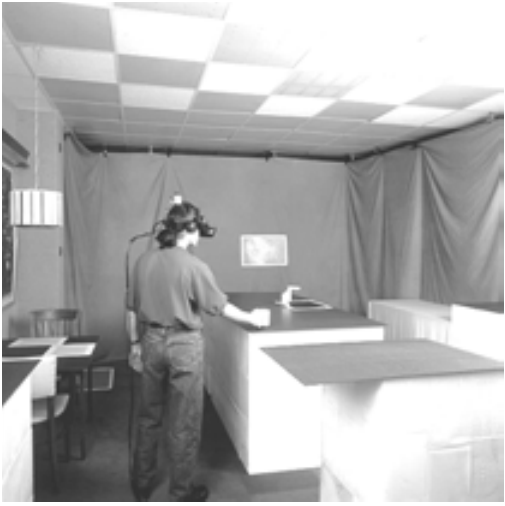
\includegraphics[width=0.3\textwidth]{figures/passiveHapticsRealRoom}\label{fig:passiveHapticsRealRoom}}
    \hfill
    \subfloat[passiveHapticsLedge][Small ledge for simulating standing at a precipice]{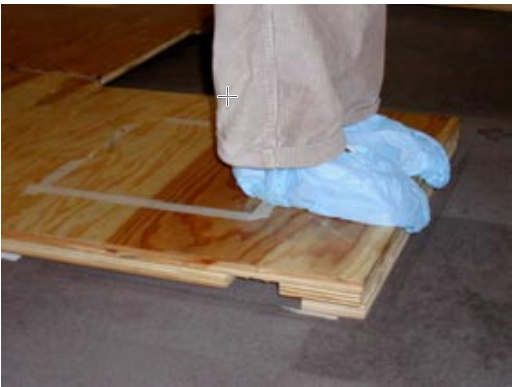
\includegraphics[width=0.3\textwidth]{figures/passiveHapticsLedge.png}\label{fig:passiveHapticsLedge}}
    \caption{Passive haptics examples}
    \label{fig:passiveHapticsPics}
\end{figure}

The complexity and amount of needed props varies. At one end of the spectrum, an entire room with most furniture was recreated using cheaply made low detail props (Figures \autoref{fig:passiveHapticsVirtualRoom} and \autoref{fig:passiveHapticsRealRoom}), on the other end, a simple wooden ledge was used to simulate standing on a precipice of a much deeper pit (Figure \autoref{fig:passiveHapticsLedge}).
\newline
This kind of setup is most likely the way to achieve maximum \gls{immersiongl} for the user, as the virtual world is essentially replicated in enough detail for adequate haptic feedback. It is however impractical for most \gls{vra} applications, as it needs to be set up and registered precisely (Insko claims a misalignment of up  to three inches could be tolerated by the user \autocite[p. ~63]{passiveHaptics}) for each virtual environment. \Gls{pha} also limits the virtual environment to something that even can be replicated well enough in reality.
\newline

A similar approach is proposed in \textit{TurkDeck: Physical Virtual Reality Based on People} \autocite{turkDeck} by Lung-Pan Cheng et al., where a team of humans are constantly instructed to construct and operate props on the fly around the user, depending on where in the virtual environment he is. It is clear that such an involved solution to \gls{pha} is highly impractical for most \gls{vra} applications.
